%Szablon przygotowany przez mgr Marcina Hanca, z drobnymi zmianami dr Michała Rena
%Master's thesis - Decompiling Android OS applications by Dawid Drozd
\documentclass[12pt,a4paper,leqno,oneside,titlepage]{book}

% (TIP) Your editor should fit this line:
%%%%%%%%%%%%%%%%%%%%%%%%%%%%%%%%%%%%%%%%%%%%%%%%%%%%%%%%%%%%%%%

%%%%%%%%%%%%%%%%%%%%%%%%%%%%%%%%%%%%%%%%%%%%%%%%%%%%%%%%%%%%%%%
%%%%%%%%%%%%%%%%%%%%%%%%%%%%%%%%%%%%%%%%%%%%%%%%%%%%%%%%%%%%%%%
%                      config
%%%%%%%%%%%%%%%%%%%%%%%%%%%%%%%%%%%%%%%%%%%%%%%%%%%%%%%%%%%%%%%
%%%%%%%%%%%%%%%%%%%%%%%%%%%%%%%%%%%%%%%%%%%%%%%%%%%%%%%%%%%%%%%


% Wczytanie pakietów: kodowania, czcionki i języki.
\usepackage[utf8]{inputenc}
\usepackage{lmodern}
\usepackage[english,polish]{babel}
% Wczytanie pakietu 'polski' w celu zapewnienia polskich nazw.
\usepackage{polski}
% Czcionki matematyczne.
\usepackage{amsfonts}
\usepackage{amsmath}

% Ładne początki rozdziałów (pakiet fncychap).
% Polecam Sonny i Conny. Bjornstrup najładniejszy, ale mi się bugował.
\usepackage[Sonny]{fncychap}
% Ładne i klikalne odnośniki.
\usepackage{url}
% Odnośniki dla adresów z polskimi znakami.
\usepackage[]{hyperref}
% Możliwość tworzenia łączonych pól (wg. rzędów) w tabelach.
\usepackage{multirow}
% Pakiet do cytowania kodów źródłowych.
\usepackage{listings}
% Pakiet do ładnego wstawiania grafik.
\usepackage{graphicx}
% Pakiet dodający możliwość wstawienia rozdziału "Akronimy".
\usepackage{acronym}
% Pakiet dodający kolory
\usepackage[usenames,dvipsnames,svgnames,table]{xcolor}
% Pakiet rozwiązujący problem z underscore w Section.
\usepackage[T1]{fontenc}
% Pakiet dodający definicje i twierdzenia.
\usepackage{amsthm}

% Custom format of ARM Assembler source code
\usepackage{package/arm-assembler-latex-listings/lstlangarm}
% Custom format for JavaScript
\usepackage{package/lstlangjavascript}
% Custom format for Diff preview
\usepackage{package/lstlangdiff}

\frenchspacing

\newcommand{\myAuthorName}{Dawid Patryk Drozd}
\author{\myAuthorName{}}
\title{Dekompilacja aplikacji działających w systemie Android OS.}

% \imod{k} Ładny zapis dzielenia modulo.
\makeatletter
\def\imod#1{\allowbreak\mkern10mu({\operator@font mod}\,\,#1)}
\makeatother

% \rom{n} Liczba n zapisana rzymsko.
\makeatletter
\newcommand*{\rom}[1]{\expandafter\@slowromancap\romannumeral #1@}
\makeatother

% Własne definicje.
% \begin{mydef}
%     Treść definicji.
% \end{mydef}
\newtheorem{mydef}{Definicja}

% Ładny sposób wstawiania cytatu rozpoczynającego rozdział.
% \begin{chapquote}{KTO}
%     CO ONA POWIEDZIAŁA?
% \end{chapquote}
\makeatletter
\renewcommand{\@chapapp}{}
\newenvironment{chapquote}[2][2em]
  {\setlength{\@tempdima}{#1}%
   \def\chapquote@author{#2}%
   \parshape 1 \@tempdima \dimexpr\textwidth-2\@tempdima\relax%
   \itshape}
  {\par\normalfont\hfill--\ \chapquote@author\hspace*{\@tempdima}\par\bigskip}
\makeatother

% Zmiana tekstów w listingach kodów źródłowych na j. polski.
\renewcommand\lstlistingname{Kod źródłowy}
\renewcommand\lstlistlistingname{Spis kodów źródłowych}

% Redefinicja Abstract'ów.
% W celu możliwości wstawienia dwóch na jedną stronę.
\newenvironment{abstractpage}
  {\cleardoublepage\vspace*{\fill}\thispagestyle{empty}}
  {\vfill\cleardoublepage}
\newenvironment{abstract}[1]
  {\bigskip\selectlanguage{#1}%
   \begin{center}\bfseries\abstractname\end{center}}
  {\par\bigskip}

% Dodatkowe definicje stylu stron.
\lstset{
  basicstyle={\small\ttfamily},
  breaklines=true,
  columns=flexible,
  frame=single
}

% ToDo marker command
\newcommand{\todo}[1]{\colorbox{yellow}{#1}}

\setlength{\oddsidemargin}{0.5in}
\setlength{\textwidth}{5.7in}
\setlength{\topmargin}{0in}
\setlength{\textheight}{8.5in}
\linespread{1.05}

%%%%%%%%%%%%%%%%%%%%%%%%%%%%%%%%%%%%%%%%%%%%%%%%%%%%%%%%%%%%%%%
%%%%%%%%%%%%%%%%%%%%%%%%%%%%%%%%%%%%%%%%%%%%%%%%%%%%%%%%%%%%%%%
%                      begin{document}
%%%%%%%%%%%%%%%%%%%%%%%%%%%%%%%%%%%%%%%%%%%%%%%%%%%%%%%%%%%%%%%
%%%%%%%%%%%%%%%%%%%%%%%%%%%%%%%%%%%%%%%%%%%%%%%%%%%%%%%%%%%%%%%

% Tu rozpoczyna się zawartość pracy!
\begin{document}

% Strona tytułowa zgodna z wymaganiami:
% http://www.wmi.amu.edu.pl/pl/prace-dyplomowe
\begin{titlepage}
\let\footnotesize\small
\let\footnoterule\relax
\let \footnote \thanks

\begin{center}
{\large \bf Uniwersytet im. Adama Mickiewicza w Poznaniu \\ Wydział Matematyki i~Informatyki \par}
\vspace{0.5cm plus 1mm minus 2mm}
{{\bf Kierunek: Informatyka} \\ \small Specjalizacja:\todo{MISSING!}\par}
\end{center}%

\vspace{1.5cm plus 1fill}
\begin{flushleft}
{\center {\bf \Large \myAuthorName{}} \\ \normalsize Nr albumu: \bf 362617\par}
\end{flushleft}
\vspace{1.5cm plus 1mm minus 2mm}

\begin{center}
{\huge\textbf{Dekompilacja aplikacji działających w systemie Android~OS}\par}
\vspace{0.5cm plus 1mm minus 2mm}
{\large Decompiling Android OS applications}
\par
\vspace{1.5cm plus 1.5fill}

\begin{flushright}\large
\begin{tabular}{l}
Praca magisterska\\[3pt]
\MakeUppercase{ }\\[3pt]
Promotor: \\[3pt]
\bfseries dr Michał Ren \\[3pt]
\end{tabular}
\end{flushright}
\vspace{4cm plus .1fill}
{\large 2017\par}
\end{center}
\end{titlepage}

% Zgłoszenie braku numerowania kolejnych stron.
\pagenumbering{gobble}

\begin{flushright}{
Poznań, dnia 25 czerwca 2017
}\end{flushright}
\begin{center}{
\par
\vspace{1.5cm plus 1.5fill}
{\large OŚWIADCZENIE}
}\end{center}
\par
\vspace{1.5cm plus 1.5fill}
Ja, niżej podpisany \myAuthorName{} student Wydziału Matematyki i~Informatyki Uniwersytetu im. Adama Mickiewicza w Poznaniu oświadczam, że przedkładaną pracę dyplomową pt: ``Dekompilacja aplikacji działających w systemie Android OS'' napisałem samodzielnie. Oznacza to, że przy pisaniu pracy, poza niezbędnymi konsultacjami, nie korzystałem z pomocy innych osób, a~w~szczególności nie zlecałem opracowania rozprawy lub jej części innym osobom, ani nie odpisywałem tej rozprawy lub jej części od innych osób.\\

Oświadczam również, że egzemplarz pracy dyplomowej w~wersji drukowanej jest całkowicie zgodny z~egzemplarzem pracy dyplomowej w~wersji elektronicznej.\\

Jednocześnie przyjmuję do wiadomości, że przypisanie sobie, w~pracy dyplomowej, autorstwa istotnego fragmentu lub innych elementów cudzego utworu lub ustalenia naukowego stanowi podstawę  stwierdzenia  nieważności postępowania w~sprawie nadania tytułu zawodowego.\\

Wyrażam zgodę na udostępnianie mojej pracy w czytelni Archiwum UAM.\\

Wyrażam zgodę na udostępnianie mojej pracy w zakresie koniecznym do ochrony mojego prawa do autorstwa lub praw osób trzecich.
\par
\vspace{1.5cm plus 1.5fill}
\begin{center}{
..............................................\\
{\footnotesize(czytelny podpis studenta)}
}\end{center}


%%%%%%%%%%%%%%%%%%%%%%%%%%%%%%%%%%%%%%%%%%%%%%%%%%%%%%%%%%%%%%%
%%%%%%%%%%%%%%%%%%%%%%%%%%%%%%%%%%%%%%%%%%%%%%%%%%%%%%%%%%%%%%%
%                      Thanks to...
%%%%%%%%%%%%%%%%%%%%%%%%%%%%%%%%%%%%%%%%%%%%%%%%%%%%%%%%%%%%%%%
%%%%%%%%%%%%%%%%%%%%%%%%%%%%%%%%%%%%%%%%%%%%%%%%%%%%%%%%%%%%%%%

\newpage

\phantom{.}

\vspace{12cm} \hspace{1cm}\phantom{.}\\
\phantom{.}\hspace{5cm}{Składam serdeczne podziękowania}\\
\phantom{.}\hspace{5cm}{doktorowi }\\
\phantom{.}\hspace{5cm}{Michałowi Renowi }\\
\phantom{.}\hspace{5cm}{za jego nieocenioną pomoc }\\
\phantom{.}\hspace{5cm}{przy pisaniu tej pracy.}\\
\phantom{.}\hspace{5cm}{}\\
\phantom{.}\hspace{5cm}{Dziękuję również}\\
\phantom{.}\hspace{5cm}{Marcinowi Hancowi za szablon i }\\
\phantom{.}\hspace{5cm}{za owocną, naukową współpracę}\\
\phantom{.}\hspace{5cm}{przy tworzeniu wyników z tej pracy.}\\


%%%%%%%%%%%%%%%%%%%%%%%%%%%%%%%%%%%%%%%%%%%%%%%%%%%%%%%%%%%%%%%
%%%%%%%%%%%%%%%%%%%%%%%%%%%%%%%%%%%%%%%%%%%%%%%%%%%%%%%%%%%%%%%
%                      Bookmarks
%%%%%%%%%%%%%%%%%%%%%%%%%%%%%%%%%%%%%%%%%%%%%%%%%%%%%%%%%%%%%%%
%%%%%%%%%%%%%%%%%%%%%%%%%%%%%%%%%%%%%%%%%%%%%%%%%%%%%%%%%%%%%%%

\newpage
% Przód pracy - spisy i abstrakty.
\frontmatter
% Spis treści ze specjalnym uwzględnieniem podkreśleń w tytułach sekcji.
\pagestyle{plain}
{
    \catcode`\_=12
    \tableofcontents
}
% Spis ilustracji.
\listoffigures
% Spis tabeli.
\listoftables
% Spis listingów kodów źródłowych.
\begingroup
\let\clearpage\relax
\lstlistoflistings
\endgroup

%%%%%%%%%%%%%%%%%%%%%%%%%%%%%%%%%%%%%%%%%%%%%%%%%%%%%%%%%%%%%%%
%%%%%%%%%%%%%%%%%%%%%%%%%%%%%%%%%%%%%%%%%%%%%%%%%%%%%%%%%%%%%%%
%                      Abstract
%%%%%%%%%%%%%%%%%%%%%%%%%%%%%%%%%%%%%%%%%%%%%%%%%%%%%%%%%%%%%%%
%%%%%%%%%%%%%%%%%%%%%%%%%%%%%%%%%%%%%%%%%%%%%%%%%%%%%%%%%%%%%%%

% Strona z abstraktami.
\begin{abstractpage}
% Abstrakt w języku polskim.
\begin{abstract}{polish}
Celem pracy jest omówienie procesu dekompilacji aplikacji mobilnych pisanych na system operacyjny Android.
Na początku poznamy budowę aplikacji androidowej. Korzystając z tej wiedzy nauczymy się obsługi narzędzi które ułatwiają proces dekompilacji. Dzięki narzędzią otrzymamy wynik desasemblacji i nauczymy się go interpretować. Z tak otrzymanego wyniku postaramy się poskładać wszystko z powrotem do działającej aplikacji. Dowiemy się jak system Android identyfikuje i weryfikuje pochodzenie aplikacji. Na koniec dowiemy się jakie niebezpieczeństwo niesie za sobą źle zabezpieczony kod aplikacji. Prześledzimy proces który utrudnia odzyskiwanie kodu źródłowego za pomocę technik odwrotnej inżynierii.
 
\end{abstract}
\smallskip
\noindent \textbf{Słowa~kluczowe:} RE, reverse engineering, inżynieria odwrotna, dekompilacja, android, apk, apktool, smali, obfuskacja, zaciemnianie kodu, dezasemblacja, deasembler, disassembler, objdump, asembler, dekompilator

%Abstrakt w języku angielskim.
\begin{abstract}{english}
\todo{translate when PL is done}
\end{abstract}
\smallskip
\noindent \textbf{Keywords:} \todo{translate when PL is done}
\end{abstractpage}

% Finally - PRACA!
\mainmatter

%%%%%%%%%%%%%%%%%%%%%%%%%%%%%%%%%%%%%%%%%%%%%%%%%%%%%%%%%%%%%%%
%%%%%%%%%%%%%%%%%%%%%%%%%%%%%%%%%%%%%%%%%%%%%%%%%%%%%%%%%%%%%%%
%                      Introduction
%%%%%%%%%%%%%%%%%%%%%%%%%%%%%%%%%%%%%%%%%%%%%%%%%%%%%%%%%%%%%%%
%%%%%%%%%%%%%%%%%%%%%%%%%%%%%%%%%%%%%%%%%%%%%%%%%%%%%%%%%%%%%%%

% Wstęp jest uwzględniony w spisie treści jako rozdział bez numeru.
\addcontentsline{toc}{chapter}{Wstęp}
\chapter*{Wstęp}

Inżynieria wsteczna (ang. \emph{reverse engineering}, w skrócie RE) jest procesem analizy budowy i sposobu działania oprogramowania. Proces ten jest często długim procesem ze względu na to, że analizujemy kod który poprzednio został przekształcony przez inne programy (kompilatory, preprocesory, itp.) do formy mniej czytelnej. Takim przykładem może być skompilowany program napisany w C++.


\lstinputlisting[language=C++, captionpos=b, belowcaptionskip=4pt, caption={Przykładowy program w C++}]{src/sample.cpp}

Uproszczony kod po odwrotnej inzynierii dla platformy ARM. 

\lstinputlisting[language={[ARM]Assembler}, captionpos=b, belowcaptionskip=4pt, caption={Zdesasemblowany przykładowy kod}]{src/sample.s}

Przykład choć krótki to już pokazuje jak mamy utrudnione zadanie. Często analizujemy kod który jest bardziej zrozumiały dla maszyny niż człowieka.

Proces inżynieri wstecznej jest dodatkowo utrudniany przez programistów którzy nie chcą by ktoś podglądał jak pewna funkcjonalność zastała zrealizowana. W tym celu stosowana jest obfuskacja kodu. Jednak inżynieria wsteczna czasem jest jedynym sposobem na dowiedzenie się jak coś działa. Przykładem może być brak kodu źródłowgo pewnej biblioteki jak i brak dokumentacji do niej. Innym przykładem może być chęć dodania lub naprawienia pewnej funkcjonalności. Producent mógł porzucić rozwój oprogramowania a nasza organizacja z pewnych powodów nie może zmienić tej biblioteki.

Celem tej pracy jest przedstawienie narzędzi jak i procesu dekompilacji zbudowanych aplikacji i ponownej kompilacji zmodyfikowanej aplikacji na system operacyjny Android.

\chapter{Jak zbudowana jest aplikacja na Android'a}
% https://en.wikipedia.org/wiki/Android_application_package
\section{Format .apk}

Rozszerzenie nazwy pliku bierze sie z \emph{Android Package Kit (APK)}.
Format pliku przypomina ten znany z plików .jar
Pliki oznaczone tym rozszerzeniem slużą do rozpowszechniania aplikacji na system android. Na skład paczki .apk wchodzą:

\begin{itemize}
\item skompilowany kod Java w formacie .dex
\item zasoby takie jak png czy mp3
\item certyfikaty
\item plik manifestu
\end{itemize}

Nazwa pliku jest dowolna pod warunkiem, że jest zakończona przez .apk
Pliki APK są pewnego roadzaju archiwum które bazuje na formacie ZIP.

\begin{figure}[h!]
	\centering
	\includegraphics[height=0.3\textheight]{img/apk_content_as_zip.png}
	\caption{Otworzony plik .apk za pomocą programu ark}
\end{figure}

Szczegółowa budowa paczki apk:
\begin{itemize}
\item \texttt{Katalog META\_INF}

\begin{figure}[h!]
	\centering
	\includegraphics[height=0.3\textheight]{img/apk_content_as_zip_meta_inf.png}
	\caption{META INF w ark}
\end{figure}

W katalogu znajduje się plik MANIFEST.MF. Plik ten zawiera metadane dotyczące zawartości paczki:

Przykład:

\begin{lstlisting}
Manifest-Version: 1.0
Built-By: Generated-by-ADT
Created-By: Android Gradle 2.3.3

Name: res/drawable-hdpi-v4/abc_list_longpressed_holo.9.png
SHA1-Digest: KQunCQh0E4bP0utgN0cHdQr9OwA=

Name: res/drawable-xxhdpi-v4/abc_ic_star_half_black_16dp.png
SHA1-Digest: EikVyBT5I7pmbJO2k8qF0V5hUc0=

Name: res/drawable-hdpi-v4/com_facebook_tooltip_black_background.9.png
SHA1-Digest: +DxTpyUKpT11iz68MG1Q0iB2EvA=

Name: res/drawable/common_google_signin_btn_icon_dark_normal.xml
SHA1-Digest: Qa00to2cn7JphS3q33GWp3lxTUs=
\end{lstlisting}

\item CERT.RSA - certyfikat aplikacji
\item CERT.SF
Lista zasobów i ich SHA-1 skład jest taki sam jak w przypadku MANIFEST.MF


\item Folder lib
Katalog opcjonalny w którym powinny znajdować się skompilowane biblioteki natywne na daną platformę np. armeabi, x86, mips

\item AndroidManifest.xml - dodatkowy plik manifestu który zawiera między innymi nazwy, wersję i prawa aplikacji. Plik ten często jest binarnym XML który łatwo zamienić na formę czytelną dla człowieka.

\item resources.arsc - plik zawierający prekompilowane zasoby takie jak binarne XML

\item folder assets
Folder który zawiera zasoby które nie są poddane dodatkowym obróbką przez proces budowania apk.

\item folder res
Folder zawiera zasoby które nie zostały przetworzone i dołączone do pliku resources.arsc

\item classes.dex Skompilowane pliki Java do formatu .dex które rozumie Dalvik virtual machine

\end{itemize}


%https://en.wikipedia.org/wiki/Dalvik_(software)
%https://source.android.com/devices/tech/dalvik/dex-format

\section{Format .dex}

W pliku classes.dex są przechowywane definicje naszych klas i wszystkich innych danych im towarzyszących.
Format ten służy do przenoszenia danych wejściowych dla Dalvik Bytecode. 

Istnieją wymogi które musi spełniać plik .dex by zostać uznany za prawidłowy.
% https://source.android.com/devices/tech/dalvik/constraints


W zapisie binarnym pliku na samym początku musi się pojawić tak zwany \verb|DEX_FILE_MAGIC| który jest zdefiniowany tak:

\begin{lstlisting}
ubyte[8] DEX_FILE_MAGIC = { 0x64 0x65 0x78 0x0a 0x30 0x33 0x38 0x00 }
                        = "dex\n038\0"
}
\end{lstlisting}

Jest on po to by mieć pewność, że odczytywny plik jest plikiem typu .dex

W tym identyfikatorze jest zawarty znak nowej lini '\\n' (0x0a) i znak końca tekstu '\\0' (0x00). Służy to tylko dodatkowym zabezpieczeniom by wykryć uszkodzenie danych.

Wartość ta też zawiera numer wersji formatu. Są to 3 cyfry pomiędzy nową linią a znakiem null. Oczywiście w calech ewolucji danego formatu.

Plik .dex jest podzielony na sekcje określone przez nagłówek.

\verb|string_ids|  W tej sekcji znajdują się wszystkie identyfikatory dla wszystkich stringów w tym pliku. Lista tych stringów musi być posortowana po nazwie przy użyciu \verb|UTF-16| nie uwzględniając ustawień lokalnych komputera. Lista jest unikatowa. To znaczy nie zawiera powtórzeń.

\verb|type_ids| Lista wszystkich typów występujących w pliku. Tych zdefiniowanych i tych zadeklarowanych. Takich jak klasy, tablice, typy primitywne. Lista ta jest posortowana po \verb|string_id| index i nie zawiera duplikatów

\verb|proto_ids|	

Opis:
	Lista wszystkich prototypów metod znajdujących się w tym pliku.
Specyfika danych:
	Lista zawiera unikaty
	Lista jest posortowana po:
		typie zwracanym (jego indeksie w \verb|type_id|
		po liście argumentów i ich \verb|type_id|

Lista wszystkich prototypów metod znajdujących się w tym pliku. Lista jest posort 


\verb|field_ids|

Opis:
	Lista wszystkich identyfikatorów pól.	
Specyfika danych:
	Lista jest posortowana po typie (jego indeksie \verb|type_id|) następnie po nazwie pola (jego indeksie \verb|string_id|)
	Lista nie zawiera duplikatów.
	
\verb|method_ids|

Opis:
	Lista wszystkich identyfikatorów metod.
Specyfika danych:
	Lista nie zawiera duplikatów.
	Lista jest posortowana po definiowanym typie (jego indeksie \verb|type_id|)
	następnie po nazwie (jego indeksie \verb|string_id|) i na koniec po prototypie metody (jego indeksie \verb|proto_id|)


Rozszerzenie nazwy pliku bierze sie z \emph{Android Package Kit (APK)}.
Format pliku przypomina ten znany z plików .jar
Pliki oznaczone tym rozszerzeniem slużą do rozpowszechniania aplikacji na system android. Na skład paczki .apk wchodzą:

\begin{itemize}
\item skompilowany kod Java w formacie .dex
\item zasoby takie jak png czy mp3
\item certyfikaty
\item plik manifestu
\end{itemize}

Nazwa pliku jest dowolna pod warunkiem, że jest zakończona przez .apk
Pliki APK są pewnego roadzaju archiwum które bazuje na formacie ZIP.

\begin{figure}[h!]
	\centering
	\includegraphics[height=0.3\textheight]{img/apk_content_as_zip.png}
	\caption{Otworzony plik .apk za pomocą programu ark}
\end{figure}

Szczegółowa budowa paczki apk:
\begin{itemize}
\item \texttt{Katalog META\_INF}

\begin{figure}[h!]
	\centering
	\includegraphics[height=0.3\textheight]{img/apk_content_as_zip_meta_inf.png}
	\caption{META INF w ark}
\end{figure}

W katalogu znajduje się plik MANIFEST.MF. Plik ten zawiera metadane dotyczące zawartości paczki:

Przykład:

\begin{lstlisting}
Manifest-Version: 1.0
Built-By: Generated-by-ADT
Created-By: Android Gradle 2.3.3

Name: res/drawable-hdpi-v4/abc_list_longpressed_holo.9.png
SHA1-Digest: KQunCQh0E4bP0utgN0cHdQr9OwA=

Name: res/drawable-xxhdpi-v4/abc_ic_star_half_black_16dp.png
SHA1-Digest: EikVyBT5I7pmbJO2k8qF0V5hUc0=

Name: res/drawable-hdpi-v4/com_facebook_tooltip_black_background.9.png
SHA1-Digest: +DxTpyUKpT11iz68MG1Q0iB2EvA=

Name: res/drawable/common_google_signin_btn_icon_dark_normal.xml
SHA1-Digest: Qa00to2cn7JphS3q33GWp3lxTUs=
\end{lstlisting}

\item CERT.RSA - certyfikat aplikacji
\item CERT.SF
Lista zasobów i ich SHA-1 skład jest taki sam jak w przypadku MANIFEST.MF


\item Folder lib
Katalog opcjonalny w którym powinny znajdować się skompilowane biblioteki natywne na daną platformę np. armeabi, x86, mips

\item AndroidManifest.xml - dodatkowy plik manifestu który zawiera między innymi nazwy, wersję i prawa aplikacji. Plik ten często jest binarnym XML który łatwo zamienić na formę czytelną dla człowieka.

\item resources.arsc - plik zawierający prekompilowane zasoby takie jak binarne XML

\item folder assets
Folder który zawiera zasoby które nie są poddane dodatkowym obróbką przez proces budowania apk.

\item folder res
Folder zawiera zasoby które nie zostały przetworzone i dołączone do pliku resources.arsc

\item classes.dex Skompilowane pliki Java do formatu .dex które rozumie Dalvik virtual machine

\end{itemize}

\todo{Dokończyć tą sekcję}

\chapter{Narzędzia do dekompilacji}

\section{apktool}

Narzędzie to służy do przeprowadzenia odwrotnej inżynierii na wskazanym pliku apk. Potrafi zdekodować źródła aplikacji do formy zbliżonej przed jej zbudowaniem. Wiele procesów zostało zautomatyzowanych takich jak zbudowanie ponowne aplikacji z zdekompilowanych źródeł. \\
\lstinline|apktool| jest otwarto źródłowym oprogramowaniem na licencji \mbox{Apache 2.0 License.} \\
\\
Kod narzędzia jest dostępny na: \url{https://github.com/iBotPeaches/Apktool} \newline
Strona narzędzia: \url{https://ibotpeaches.github.io/Apktool/}
\newline
\newline
Aplikacja jest napisana w języku Java dzięki czemu działa bezproblemowo na większości systemach operacyjnych. Jest to aplikacja bez interfejsu graficznego. Działa w konsoli.
\newline
\subsection{Dekompilacja}
Przykład użycia zostanie zaprezentowany na przykładowej aplikacji. Zakładając, że mamy już dostępną naszą \lstinline|.apk|\\
\begin{lstlisting}[language=bash]
{master} ~/Projects/UAM/
$ cd apktool
{master} ~/Projects/UAM/msc/apktool
$ ./apktool d ../sample-android-app/Thesis/app/app-release.apk 
I: Using Apktool 2.2.3 on app-release.apk
I: Loading resource table...
I: Decoding AndroidManifest.xml with resources...
I: Loading resource table from file: /home/gelldur/.local/share/apktool/framework/1.apk
I: Regular manifest package...
I: Decoding file-resources...
I: Decoding values */* XMLs...
I: Baksmaling classes.dex...
I: Copying assets and libs...
I: Copying unknown files...
I: Copying original files...
\end{lstlisting}
Dzięki tej komendzie uzyskamy źródła z naszej aplikacji. 
\begin{figure}[h!]
	\centering
	\includegraphics[height=0.3\textheight]{img/apktool/sample_apk.png}
	\caption{Wynik pracy \lstinline|apktool d app-release.apk|}
\end{figure}
\begin{itemize}
\item{Folder smali}\\
Zawiera odzyskane inżynierią wsteczną kody źródłowe naszej aplikacji. Kody jednak nie będą w języku Java a w Smali. Smali jest omówiony w \ref{smali}.
\item{Folder original}\\
Zawiera oryginalne źródła z naszego \lstinline|.apk| takie jak oryginalny \lstinline|AndroidManifest.xml| czy  \lstinline|META-INF|
\item{Folder lib}\\
Zwiera natywne biblioteki wykorzystywane przez aplikację. W naszym przykładzie jest to skompilowana dynamiczna biblioteka z jedną prostą funkcją. Oby odzyskać kod natywny musielibyśmy sięgnąć do innych narzędzi.
\item{Folder res}\\
Zawiera wszystkie oryginalne zasoby naszej aplikacji które zostały wcześniej przetworzone i w odpowiedni sposób upakowane.
\item{apktool.yml}\\
Plik z metadanymi od apktool.
\item{AndroidManifest.xml}\\
Zdekodowany \lstinline|AndroidManifest.xml|.
\end{itemize}
%
\begin{figure}[h!]
	\centering
	\includegraphics[width=1\textwidth]
	{img/apktool/sample_diff_manifest.png}
	\caption{Diff między AndroidManifest.xml z źródeł a odzyskanym z pliku .apk}
\end{figure}
%
\subsection{Budowanie z powrotem}
Aplikację możemy zbudować ponownie z naszych zasobów. Przykład tego zastosowania znajduje się poniżej.

\begin{lstlisting}[language=bash]
{master} ~/Projects/UAM/msc/apktool
$ ./apktool b ./app-release/
I: Using Apktool 2.2.3
I: Checking whether sources has changed...
I: Smaling smali folder into classes.dex...
I: Checking whether resources has changed...
I: Building resources...
I: Copying libs... (/lib)
I: Building apk file...
I: Copying unknown files/dir...
\end{lstlisting}
W taki sposób otrzymamy znowu zbudowaną aplikację jednak nie będzie ona podpisana tym samym kluczem. Jaki wpływ na aplikację ma podpisaniem kluczem jest omówione w \ref{signing} rozdziale.

\section{dex2jar}
% https://github.com/pxb1988/dex2jar
Narzędzie to służy do przeprowadzenia odwrotnej inżynierii na pliku \lstinline|.dex|. Program jest troszkę mniej wygodny w porównaniu do apktool ponieważ sami musimy wywołać odpowiednie skrypty i wydobyć to co chcemy.

\begin{lstlisting}[language=bash]
{master} ~/Projects/UAM/msc
$ cd dex2jar/dex2jar-2.0
{master} ~/Projects/UAM/msc/dex2jar/dex2jar-2.0
$ ./d2j-dex2smali.sh ../../sample-android-app/Thesis/app/app-release.apk
baksmali ../../sample-android-app/Thesis/app/app-release.apk -> app-release-out
\end{lstlisting}
W taki sposób uzyskamy nasze zdekompilowane pliki \lstinline|.smali|. Narzędzie to też umożliwia odzyskanie plików \lstinline|.class| które później mogą posłużyć do analizy przez inne programy np. \verb|JD-GUI|

\section{apkToJava}
% https://github.com/ajitsing/apkToJava
\todo{Czy warto opisywać to narzędzie?}

\section{Inne}
Oczywiście narzędzi istnieje znacznie więcej. Ja w mojej pracy jednak skupiłem się na apktool ze względów na przyjemne użytkowanie i duże społeczeństwo zebrane wokół tego narzędzia.\\
Jednym z narzędzi wartych zainteresowania może być \href{http://vaibhavpandey.com/apkstudio/}{apkstudio}. Narzędzie działa to we współpracy z apktool jednak daje nam łatwy edytor dla developera.

%- Zabezpieczenia przed modyfikowaniem aplikacji (podpisywanie apki certyfikatem,nazwa package apki)

\chapter{Identyfikacja i weryfikowanie aplikacji}

W systemie Android możemy wydzielić 2 sposoby weryfikacji aplikacji. Sposoby te służą do identyfikacji aplikacji wśród wszystkich innych aplikacji zainstalowanych w systemie.

\section{Nazwa paczki}
Nazwa paczki aplikacji jest podstawowym sposobem na zidentyfikowanie aplikacji w całym systemie. Założenie jest proste. Nazwa aplikacji musi być unikatowa w skali systemu. Przez co jednocześnie nie możemy mieć aplikacji o takiej samej nazwie paczki. Oczywiście w sklepie z aplikacjami Google Play ta zasada również obowiązuje. Jednak w naszym systemie możemy mieć zupełnie inną aplikację niż ta która znajduje się w sklepie a będą miały taką samą nazwę paczki. Oczywiście nie będziemy mogli zainstalować ze sklepu takiej aplikacji póki nie usuniemy jej pierw z systemu.\\
Jest to bardzo prymitywna metoda identyfikacji którą łatwo oszukać i podszyć się pod inną aplikację. Obrona przed tego typem oszustwa poruszymy w \ref{signing}. Dobrą praktyką i ogólnie przyjętą konwencja jest by nazwa paczki była odwróconą domeną. Tak samo jak to ma miejsce w zwykłym nazewnictwie paczek przy projektach Javowych.
\begin{center}
	\centering	\includegraphics[height=0.3\textheight]
	{img/signing/google_play_app_name.png}
\end{center}
Na powyższym rysunku możemy zobaczyć nazwę paczki która jest bezpośrednio widoczna w URL strony. Więc na tej podstawie możemy też dokonać wstępnej weryfikacji.
\begin{center}
	\includegraphics[height=0.3\textheight,keepaspectratio]
	{img/signing/two_same_aps.png}
\end{center}
Na powyższym rysunku możemy zobaczyć, że zostały zainstalowane dwie takie same aplikacje. Oczywiście zgodnie z zasadą co służy do identyfikacji aplikacji jest nazwa paczki. W tym przypadku nazwa aplikacji i ikonka są takie same. Różnią się tylko nazwą paczki:
\begin{lstlisting}
com.f2zentertainment.pandemic
com.f2zentertainment.pandemic.qa
\end{lstlisting}
Podsumowując nazwa paczki służy tylko identyfikacji. Tak jak w bazie danych \verb|ID| identyfikuje nam wiersz. 

\section{Cyfrowy podpis}
\label{signing}
% https://developer.android.com/studio/publish/app-signing.html
% https://source.android.com/security/apksigning/
% Różnica między certyfikatem a kluczem 
% https://pl.wikipedia.org/wiki/Certyfikat_klucza_publicznego
Wymogiem Android'a jest by aplikacje były cyfrowo podpisane certyfikatem przed ich zainstalowaniem. Mamy dwa klucze publiczny i prywatny. Klucz publiczny jest dołączany do naszego \lstinline|.apk|. Dzięki temu w przyszłości będzie łatwo stwierdzić od kogo pochodzi nowa aplikacja czy też aktualizacja. Narzędzie do podpisywania aplikacji (\lstinline|apksigner|) na Android'a pracuje na pliku \lstinline|.keystore|. Jest to binarny format który zawiera jeden lub wiele prywatnych kluczy. 
\begin{figure}[h!]
	\centering
	\includegraphics[width=1\textwidth,keepaspectratio]
	{img/signing/appsigning_selfmanagediagram_2x.png}
	\caption{Podpisanie aplikacji przez Developera}
\end{figure}
Klucze są zabezpieczone dodatkowymi hasłami w pliku. Jeśli zgubimy lub utracimy nasz klucz to nie będziemy w stanie aktualizować naszej aplikacji użytkownikom. Jak wcześniej było wspomniane, aplikacja musi być podpisana tym samym kluczem by system uznał ją jako aktualizację czy też autentyczna aplikację od danego twórcy.\par
Dekompilowane przez nas aplikację możemy podpisać naszym kluczem co pozwoli nam na instalację tak zmodyfikowanej aplikacji. Jednak jeśli chcielibyśmy aby system potraktował tak zmodyfikowaną aplikację jako aktualizację to już się to nie powiedzie bo poprzednia aplikacja była podpisana innym kluczem.\par
Podpisana aplikacja służy jeszcze Androidowi do identyfikacji i tworzenia użytkowników w których obrębie działa aplikacja. Aplikacje podpisane tym samym kluczem mają możliwość współdzielenia użytkownika co za tym idzie, aplikację mogą współdzielić dane bez potrzeby tworzenia skomplikowanych interfejsów.\par
Android posiada dwa sposoby podpisywania aplikacji:\par
\begin{itemize}
\item{JAR signing (v1 scheme)}\par
Metoda ta bazuje na innej metodzie podpisywaniu pliku JAR. Pliki charakterystyczne dla tego sposoby podpisywania są pliki w katalogu \verb|META-INF| 
\par
\begin{figure}[h!]
	\centering
	\includegraphics[width=1\textwidth,keepaspectratio]
	{img/signing/apk_signed_v1_vs_signed_with_v2.png}
	\caption{Przykładowy APK. Po lewej APK podpisany metodą v1, po prawej metodą v2}
\end{figure}
% https://source.android.com/security/apksigning/
% https://docs.oracle.com/javase/8/docs/technotes/guides/jar/jar.html#Signed_JAR_File
Wadami tej metody jest, że nie chroni pewnych obszarów APK przed modyfikacją takich jak metadane. Dodatkowo program weryfikujący musi przetworzyć sporo nie zweryfikowanych danych by je zweryfikować. Takie podeście tworzy furtkę do ataku. Dodatkowo trzeba odpakować wszystkie zasoby co niestety jest też czasochłonne.
\item{APK Signature Scheme v2 (v2 scheme)}
Metoda ta dostępna jest od Android'a 7.0. Zawartość naszego APK przechodzi przez funkcję hashującą co następnie zostaje podpisane. Taki blok zostanie następnie dodany do naszego APK. Podczas walidacji APK jest traktowane jako kontener i sprawdza hashe wszystkich plików wewnątrz APK, łącznie z metadanymi. Nowy format jest kompatybilny wstecz. Starsze urządzenia zignorują dodatkowe dane i wykonają sprawdzanie według metody v1. Oczywiście aplikacja musi być podpisana dwoma sposobami.
\end{itemize}

\begin{figure}[h!]
	\centering
	\includegraphics[width=1\textwidth,keepaspectratio]
	{img/signing/apk-validation-process.png}
	\caption{Weryfikacja podpisu APK}
\end{figure}

\chapter{Wynik desasemblacji}

\begin{figure}[h!]
	\centering
	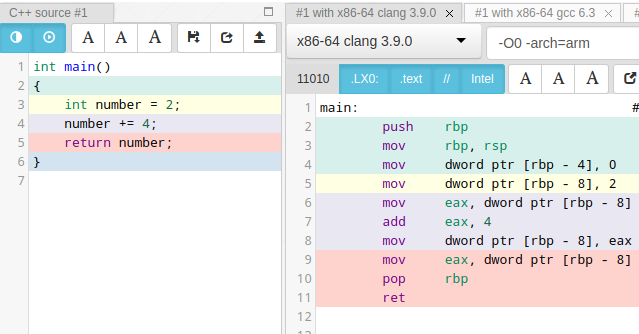
\includegraphics[height=0.3\textheight]{img/Screenshot_godbolt_org-sample.png}
	\caption{Wygenerowany przykład z strony \url{godbolt.org}}
\end{figure}

\section{SMALI}
\label{smali}
\todo{TODO}
\section{Dalvik/ART bytecode}
\todo{TODO}

\chapter{Sposoby ochrony przed desasemblacją}
% https://www.owasp.org/images/0/08/OWASP_SCP_Quick_Reference_Guide_v2.pdf
Naturalnym zjawiskiem na atak jest obrona. Mając takie proste w użyciu narzędzia do RE naturalne jest, że powstały techniki utrudniające RE. Oczywiście wykorzystano w tym kierunku wiedzę z innych technologi gdzie ów problemy występują od dziesiątek lat. Temat jest na tyle szeroki, że poruszę tylko te sposoby które są powszechnie stosowane w tworzeniu aplikacji na Android'a i są stosunkowo tanie/proste do wdrożenia. Większą bazę wiedzy na temat zabezpieczenia kodu przez inżynierią odwrotną można znaleźć na stronie \hyperlink{https://www.owasp.org/index.php/OWASP_Reverse_Engineering_and_Code_Modification_Prevention_Project}{OWASP}.
% https://stackoverflow.com/questions/43601498/protect-android-app-from-reverse-engineering
% http://resources.infosecinstitute.com/android-hacking-and-security-part-18-introduction-to-reverse-engineering/
\section{Obfuskacja}
% https://pl.wikipedia.org/wiki/Zaciemnianie_kodu
Technika ta często też nazywana zaciemnianiem kodu czy potocznie kolorowaniem. Jest to jedna z podstawowych technik \textbf{utrudniających} odzyskanie kodu. Technika ta polega na zamienianiu czytelnych dla programisty wyrażeń na wyrażenia krótkie i nie czytelne dla ludzi napisy. Oczywiście z zachowaniem poprawności i zasad danego języka. Więc technika ta nie modyfikuje zachowania kodu a jedynie sprawia, że reprezentacja kodu staje się mniej czytelna dla ludzi. Napisałem, że jest to technika utrudniająca inżynierię wsteczną a nie zapobiegającą bo jej celem jest tylko utrudnienie odczytania kodu. Przez co proces staje się bardziej czasochłonny. Oczywiście mocno zdeterminowanego napastnika to nie zniechęci.\par
Jako przykład posłuży nam kod napisany w języku JavaScript który poddamy obfuskacji. W języku Java było by to jeszcze bardziej przekształcone ze względu na transformację do kodu bajtowego.
%
\lstinputlisting[language=JavaScript, captionpos=b, belowcaptionskip=4pt, caption={Przykładowy program w JavaScript}]{src/obfuscation_source.js}
%
\lstinputlisting[language=JavaScript, captionpos=b, belowcaptionskip=4pt, caption={Kod poddany obfuskacji w JavaScript}]{src/after_obfuscation_source.js}
%
\par Oczywiście skuteczność jak i wymyślność naszego obfuskatora zależy od jego twórcy. Powyższy kod możemy jeszcze bardziej sprawić brzydszym.
%
\lstinputlisting[language=JavaScript, captionpos=b, belowcaptionskip=4pt, caption={Kod poddany obfuskacji w JavaScript}]{src/after_obfuscation_2_source.js}
%
\par Powyższe przykłady kodów zostały poddane tylko transformacją które nie zmieniły sposobu działania. Robią dokładnie to samo, zostały tylko zapisane w innych formach. W takich formach które dla człowieka utrudniają znacząco zrozumienie jego działania.
\par
Na przykładzie pokaże jak wygląda dekompilacja kodu w języka Java z obfuskacją i bez niej.
%
\lstinputlisting[language=Java, captionpos=b, belowcaptionskip=4pt, caption={Prosta implementacja listy w języku Java}]{src/java_sample/SampleJavaCode.java}
%
Powyższy kod skompilujemy i otrzymamy pliki \lstinline|.class|, każdy plik dla struktury i jeden główny.
%
\begin{figure}[h!]
	\centering
	\includegraphics[height=0.3\textheight]
	{img/secure_desasembly/compiled_sample_java.png}
	\caption{Wygenerowane pliki za pomocą komendy: \lstinline|javac SampleJavaCode.java|}
\end{figure}
%
Najbardziej interesującym nas plikiem jest \lstinline|SampleJavaCode$ForwardListImplementation.class| bo jesteśmy ciekawi jak ktoś zaimplementował ów strukturę danych.  Załóżmy, że otrzymaliśmy aplikację od kolegi który wszystko spakował w JAR'a. Po otworzeniu JAR'a zobaczylibyśmy wszystkie te pliki które widzimy na zdjęciu. Więc już sama nazwa nam wskazuje gdzie mamy szukać implementacji. Ironią losu jest taka, że im lepszej jakości ktoś napisał kod i nie poddał go obfuskacji tym prościej atakującemu będzie znaleźć to czego szuka. Oczywiście plik \lstinline|.class| jest plikiem z kodem bajtowym i czytanie go nic nam nie da więc musimy go pierw zdekompilować. Dla uproszczenia procesu skorzystamy z dekompilatora online \hyperlink{http://www.javadecompilers.com/processing}{javadecompilers.com}.
%
\lstinputlisting[language=diff, captionpos=b, belowcaptionskip=4pt,
caption={Różnica między kodem źródłowym z kodem który został odzyskany z dekompilacji. Uzyskane za pomocą komendy: \lstinline|diff -u SampleJavaCode.java SampleJavaCode_decompiled.java > SampleJavaCode_decompile.diff|}]
{src/java_sample/SampleJavaCode_decompile.diff}
%
\par
Różnica wydaje się nie znacząca a przynajmniej nie utrudnia nam to za bardzo analizowania ów kodu. Jednak jeśli nasz kod poddamy obfuskacji to nasz przykładowy JAR zostanie zmodyfikowany i nawet dzięki temu zmniejszy się rozmiar JAR'a z 2.6 KB na 1.6 KB.
%
\begin{figure}[h!]
	\centering
	\includegraphics[height=0.3\textheight]
	{img/secure_desasembly/sample_obfuscation.png}
	\caption{JAR przed obfuskacją i po obfuskcaji za pomocą narzędzia proguard}
\end{figure}
%
JAR po poddaniu obfuskcaji pozmieniał nazwy plików więc już znacznie ciężej znaleźć nas interesujący plik. Dodatkowo zdekompilowany nasz kod zmienił trochę hierarchię naszych struktur co też może dodatkowo utrudnić nam analizę.
%
\lstinputlisting[language=Java, captionpos=b, belowcaptionskip=4pt,
caption={Plik \lstinline|a.java| czyli odpowiednik \lstinline|class SampleJavaCode|}]
{src/java_sample/decompiled_after_obfuscation/a.java}
%
%
\lstinputlisting[language=Java, captionpos=b, belowcaptionskip=4pt,
caption={Plik \lstinline|b.java| czyli odpowiednik \lstinline|class ForwardListImplementation|}]
{src/java_sample/decompiled_after_obfuscation/b.java}
%
%
\lstinputlisting[language=Java, captionpos=b, belowcaptionskip=4pt,
caption={Plik \lstinline|c.java| czyli odpowiednik \lstinline|class Node|}]
{src/java_sample/decompiled_after_obfuscation/c.java}
%
%
\lstinputlisting[language=Java, captionpos=b, belowcaptionskip=4pt,
caption={Plik \lstinline|d.java| czyli odpowiednik \lstinline|interface List|}]
{src/java_sample/decompiled_after_obfuscation/d.java}
%
\par
Kody zostały lekko zmodyfikowane przeze mnie. Poprawiłem formatowanie kodu by można było go łatwiej czytać. Skorzystałem z autofrmatera kodu dostępnego w IDE Eclipse.

\section{Proguard}
% https://www.guardsquare.com/en/proguard
% https://www.guardsquare.com/en/proguard/manual/examples#application
% http://www.javadecompilers.com
% https://en.wikipedia.org/wiki/ProGuard_(software)
Progauard jest narzędziem które potrafi zmniejszyć, zoptymalizować i zaciemnić kod w języku Java. Jest darmowym narzędziem na licencji \href{https://en.wikipedia.org/wiki/GNU_General_Public_License#Version_2}{GPL v2}. Potrafi zoptymalizować kod bajtowy np. przez usunięcie nie używanego kodu.\par
Narzędzie zostało to wykorzystane w sekcji o obfuskacji. Proguard jest częścią narzędzi do budowania aplikacji na Android'a i domyślnie jest włączony dla aplikacji w trybie release. Oczywiście w naszym projekcie możemy skonfigurować to narzędzie za pomocą plików konfiguracyjnych tak by realizowało mu powierzone zadania np. zaciemniania kodu.\par
Wadą tego narzędzia jak i zarazem powodem dla którego developerzy je wyłączają jest modyfikowanie stosu wywołań (ang. stack trace) przez zmiany nazw naszych metod czy klas.
%
\begin{lstlisting}[caption={Przykładowy wyjątek dla nie zaciemnionego kodu}]
Exception in thread "main" java.lang.IndexOutOfBoundsException
        at SampleJavaCode$ForwardListImplementation.insert(SampleJavaCode.java:37)
        at Test.main(Test.java:6)
\end{lstlisting}
%
\begin{lstlisting}[caption={Przykładowy wyjątek dla kodu który został zaciemniony}]
Exception in thread "main" java.lang.IndexOutOfBoundsException
        at b.a(Unknown Source)
        at TestObfuscated.main(TestObfuscated.java:6)
\end{lstlisting}
%
W powyższym przykładzie mamy dosyć małą głębokość wywołań co nie utrudnia nam znacząco jego interpretację. Jednak problem znacząco wzrasta im mamy dłuższy stos wywołań.\par
Jak już było wspomniane możemy konfugirować proguarda by nie zaciemniał kodu. Jednak dla nas nie jest to koniecznie dobre rozwiązanie. Oczywiście proguard rozwiązuje ten problem i wytwarza nam plik z mapowaniem starych identyfikatorów na nowe tak byśmy mogli po naszej stronie w prawidłowy sposób odczytywać stos wywołań.
%
\lstinputlisting{src/java_sample/mapping.config}
%
\par
Jednak developer sporo musi często sam skonfigurować. Do tego dochodzą problemy z wywołaniami przez refleksję czy wywołania natywnego kodu (Java Native Interface). Suma tych problemów często przewyższa zysk z obfuskacji kodu i nikt nie chce poświęcać na to czasu.

\section{Natywny kod}
Często prostą i polecaną techniką jest ukrycie krytycznych części kodu w natywnym kodzie. Przykładem może być przepisany fragment kodu do C++. Dzięki czemu takiego kodu nie będzie mogła odczytać byle to początkująca osoba która nauczyła się używać apktool'a czy innego tego typu narzędzia. W takim przypadku będzie potrzebna nisko poziomowa wiedza jak i znajomość danej platformy.\par
Takie rozwiązanie jednak ma też i swoje wady. Developer który będzie tego sposobu używał też musi wiedzieć jak to zaimplementować by nie wywołać tym sposobem nadmiarowej ilości błędów. Dochodzą też problemy związane z przekazywaniem informacji/danych między kodem napisanym w Javie a np C/C++. Oczywiście wykorzystanie natywnego kodu komplikuje nam zaciemnianie kodu. Sposób ten jak i obfuskacja jednak nie służą zabezpieczeniu naszego kodu a tylko utrudnieniu napastnikowi odczytania i przeanalizowania naszej implementacji.

\section{Szyfrowanie}
% http://www.javaworld.com/article/2077342/core-java/cracking-java-byte-code-encryption.html?page=2
W poprzednich sekcjach były poruszone tylko utrudnienia jakie możemy wprowadzić w naszym programie by kod nie został odczytany/zinterpretowany. Kolejnym sposobem na znacząco utrudnienie odzyskania kodu było by szyfrowanie naszych plików. Dzięki temu aplikacja była by tylko odszyfrowana w czasie działania aplikacji. Oczywiście dla zwiększenia bezpieczeństwa klucz deszyfrujący może być dostarczany z zewnętrznego nośnika np. z serwera.
\par
Oczywiście ta technika też nie jest idealna i jeśli ktoś będzie bardzo zawzięty i będzie miał dużo czasu to też uda mu się ominąć to zabezpieczenie. Główną zmianą jaką developer musiał by wprowadzić by wykorzystać ów metodę jest napisanie własnego ClassLoader'a. Taka klasa wiedziała by jak stworzyć instancje naszej klasy by móc z niej skorzystać. Oczywiście nie musimy szyfrować całej aplikacji a tylko części najbardziej wrażliwe tak jak miało to miejsce z wykorzystaniem kodu natywnego.

\section{Inne}
Inne techniki często bazują na bezpośrednim ataku w narzędzia których się używa do odwrotnej inżynierii.
\\
\todo{Opisać tutaj przykłady takich technik z przykładowym atakiem}
\todo{serio nie istnieją lepsze techniki ?}

\chapter{Niebezpieczeństwa źle zabezpieczonego kodu}
%- Zabezpieczenia / Niebezpieczeństwa. Np wstrzykiwanie w zapytania do serwera. (Ogólnie omówić czemu warto/trzeba zabezpieczyć kod przed dekompilacją)
% http://esec-lab.sogeti.com/static/publications/10-hitbkl-drm.pdf
Źle zabezpieczonego lub też w ogóle nie zabezpieczonego kodu. Często developerzy nie myślą o skutkach jakie niesie z sobą odwrotna inżynieria na ich aplikacjach. Często API serwisów internetowych nie jest zabezpieczone w żaden sposób i to właśnie z pomocą inżynierii wstecznej można uzyskać pełne REST'owe API danego serwisu.
\par
Jako przykładem posłużę się trzema aplikacjami w przypadku których odwrotna inżynieria może nam dostarczyć wielu ciekawych informacji. W ich przypadku włączenie zaciemniania kodu nie przyniosło zadowalających wyników. Jednak nie należy winić obfuskacji samej w sobie a zwykłe niedbalstwo ze strony programistów.

\section{Hasła bez obfuskacji}
% https://docs.google.com/presentation/d/1EI8cfZ5Vl5fiC03C5dogrM5GRHfcLTechk1OHBnAy6E/edit#slide=id.g10f8594d37_0_334
\todo{Czy podawać nazwy aplikacji ?}
\\
Aplikacja która dostarcza nam oferty zniżkowe typu kupony, rabaty dzięki którym możemy coś kupić. Pierwszym sposobem by zagwarantować sobie dostęp do ogromnej ilości zniżek/kuponów było by wydobycie ich z API twórcy aplikacji. Możemy taki proces zautomatyzować co powinno nam dostarczyć łatwy dostęp do kodów rabatowych. Wystarczy przy użyciu narzędzia np. wireshark nasłuchać w sieci lokalnej jakie metody API są odpytywane i zreprodukować zapytania. Na szczęście twórca aplikacji zabezpieczył się przez użycie hasła do API które jest ukrytn w zapytaniu HTTPS więc nie możemy go w łatwy sposób wydobyć. Tutaj przychodzi nam na pomoc RE. Przy użyciu narzędzia apktool uzyskujemy kod który nie jest zaciemniony. Prosto możemy zgadnąć jak ktoś trzyma hasło w kodzie o ile stosuje dobre praktyki programistyczne. W tym przypadku jest to strzał w dziesiątkę. Wystarczy przeszukać kod pod frazą "password"
%
\begin{figure}[h!]
	\centering
	\includegraphics[height=0.3\textheight]
	{img/why_secure/find_password.png}
	\caption{Szukanie hasła w źródłach aplikacji}
\end{figure}
%
Dzięki prostemu, szybkiemu przeszukaniu kodu możemy zerknąć bezpośrednio do pliku w którym znajduje się odpowiedź na nasze pytanie.
%
\begin{figure}[h!]
	\centering
	\includegraphics[height=0.3\textheight]
	{img/why_secure/password_in_smali.png}
	\caption{Ukryte hasło}
\end{figure}
%
\section{Generator tokenów}
Aplikacje mobilne coraz częściej służą jako metoda podwójnego uwierzytelniania czy też identyfikowania użytkownika bo ciężko jest by ktoś posiadał tysiąc komórek. W przypadku firmy Steam która prawdopodobnie miała dosyć automatycznych botów które się rejestrowały w serwisie i wykonywały pewne akcje, więc zdecydowali się wyłączyć uwierzytelnianie kodem na e-maila i zmusić użytkowników do korzystania z generatora tokenów z ich aplikacji.
%
\begin{figure}[h!]
	\centering
	\includegraphics[height=0.3\textheight]
	{img/why_secure/steam_tokener.png}
	\caption{Generator tokenów w aplikacji Steam}
\end{figure}
%
Więc od teraz wszystkie boty musiał by posiadać swoją instancję aplikacji Steam by móc generować tokeny. Jednak znów wystarczyło wykorzystać inżynierię zwrotną by wydobyć algorytm który był odpowiedzialny za generowanie tokenów. Oczywiście w tym przypadku aplikacja była poddana obfuskacji i nie jest tak prosto znaleźć ten algorytm gdzie był ukryty. Oczywiście po żmudnej analizie nie czytelnego kodu i analizowaniu wykonywania udało się odnaleźć ów algorytm i go wyodrębnić do przyjaznej skryptowej postaci. Wystarczyło ów algorytm tylko odpowiednio zainicjalizować i gotowe. Nie potrzebujemy do tego dedykowanej aplikacji.

\section{Blokady}
Aplikacje często posiadają blokady czy pewne inne nieudogodnienia np. dla użytkowników którzy mają odblokowane urządzenie (rooted device). W przypadku aplikacji Starbucks aplikacja ta na samym starcie aplikacji sprawdza czy urządzenie jest zrootowane i jeśli tak to kończy swoje działanie, uniemożliwiając korzystanie z niej. 
%
\begin{figure}[h!]
	\centering
	\includegraphics[width=0.6\textwidth]
	{img/why_secure/device_rooted_message.png}
	\caption{Komunikat od aplikacji Starbucks}
\end{figure}
%
Korzystając z RE możemy odzyskać kod ów aplikacji i usunąć sprawdzanie dzięki czemu aplikacja będzie dla nas działać. Kod aplikacji został poddany zaciemnieniu przez co ciężko było znaleźć gdzie jest sprawdzany ten warunek. Z pomocą przyszedł komunikat który wyświetlał się nam na ekranie. Jeżeli wyszukaliśmy ów tekst w plikach aplikacji to znajdziemy początek nici po której dojdziemy do naszego kłębka. 
%
\begin{figure}[h!]
	\centering
	\includegraphics[width=1\textwidth]
	{img/why_secure/search_for_message.png}
	\caption{Szukanie wiadomości prezentowanej przez aplikację}
\end{figure}
%
Dzięki prostemu wyszukaniu gdzie jest używany komunikat jesteśmy w stanie precyzyjnie znaleźć miejsce naszej blokady i je wyłączyć.
%
\begin{figure}[h!]
	\centering
	\includegraphics[width=1\textwidth,keepaspectratio]
	{img/why_secure/disable_block.png}
	\caption{Wyłączenie blokady sprawdzającej czy urządzenie jest zrootowane}
\end{figure}
%
Tego typu blokady tyczą się również sprawdzania czy użytkownik używa płatnej aplikacji i czy dana funkcjonalność powinna być odblokowana.

\chapter{Projekt}
\todo{Propozycje projektu}\\
\todo{1. Aplikacja do odbierania prawa dostępu do internetu innym aplikacja zainstalowanym na telefonie użytkownika}
\todo{2. Biblioteka do zabezpieczania fragmentów kodu przed RE wykorzystująca szyfrowanie}
\todo{3. TBC}

%\chapter{Bibliografia}
\newpage
% Dodanie wpisu Bibliografia do Spisu Treści.
\addcontentsline{toc}{chapter}{Bibliografia}
% Styl bibliografii: unsrt lub plain
\bibliographystyle{plain}
\bibliography{bibliografia}

%%%%%%%%%%%%%%%%%%%%%%%%%%%%%%%%%%%%%%%%%%%%%%%%%%%%%%%%%%%%%%%
%%%%%%%%%%%%%%%%%%%%%%%%%%%%%%%%%%%%%%%%%%%%%%%%%%%%%%%%%%%%%%%
%%%%%%%%%%%%%%%%%%%%%%%%%%%%%%%%%%%%%%%%%%%%%%%%%%%%%%%%%%%%%%%
%%%%%%%%%%%%%%%%%%%%%%%%%%%%%%%%%%%%%%%%%%%%%%%%%%%%%%%%%%%%%%%
%%%%%%%%%%%%%%%%%%%%%%%%%%%%%%%%%%%%%%%%%%%%%%%%%%%%%%%%%%%%%%%
%%%%%%%%%%%%%%%%%%%%%%%%%%%%%%%%%%%%%%%%%%%%%%%%%%%%%%%%%%%%%%%
%%%%%%%%%%%%%%%%%%%%%%%%%%%%%%%%%%%%%%%%%%%%%%%%%%%%%%%%%%%%%%%
%%%%%%%%%%%%%%%%%%%%%%%%%%%%%%%%%%%%%%%%%%%%%%%%%%%%%%%%%%%%%%%

% Spis akronimów użytych w pracy
\chapter*{Akronimy}
\begin{acronym}
\acro{KISS}{Keep It Simple Stupid}
\acro{RE}{reverse engineering}
\acro{IT}{Information Technology}
\acro{APK}{Android Package}
\end{acronym}
\end{document}
